\begin{frame}{Méthode d'expérimentation}
    \begin{itemize}
        \item Utilisation de bases de connaissance avec un petit nombre de faits et de règles mais générant beaucoup de redondances ;
        \item Nous avons retenu le nombre de faits produits à chaque étape réalisée lors de la saturation, le temps pris et la cause d'arrêt de la saturation (arrêt normal, \textit{timeout}, trop de faits) ;
        \item Comparaison entre les implémentations de Graal et les nôtres.
    \end{itemize}
    
    
    %Pour nos test nous avons utilisé des bases de connaissances avec un petit nombre de faits et de règles mais générant de nombreuse redondances. 
    %Pour comparer nos résultats nous avons retenu le nombre de faits produits, le nombre d'étapes réalisé lors de la saturation et le temps pris.
    %Nous avons ensuite comparer les résultats obtenue par les algorithme déjà présent dans Graal et nos propres algorithmes.
\end{frame}


\begin{frame}{Quelques résultats d'expérimentations}
    \begin{itemize}
        \item Nouveau \textit{restricted chase} souvent un peu plus rapide ;
        \item<2-> Dans certains cas le \textit{core chase} est le plus rapide des \textit{chases}
        \item<3-> Détection d'un bug dans le \textit{restricted chase} dans \textit{Graal}.
    \end{itemize}
    \begin{center}
    \only<1>{
        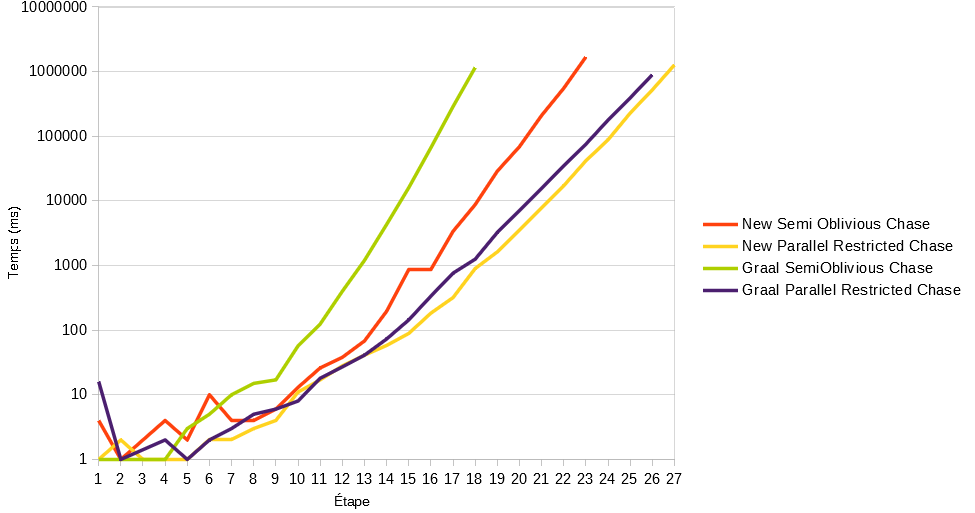
\includegraphics[width=0.8\textwidth]{img/exampleoldnew.png}
    }
    \only<2>{
        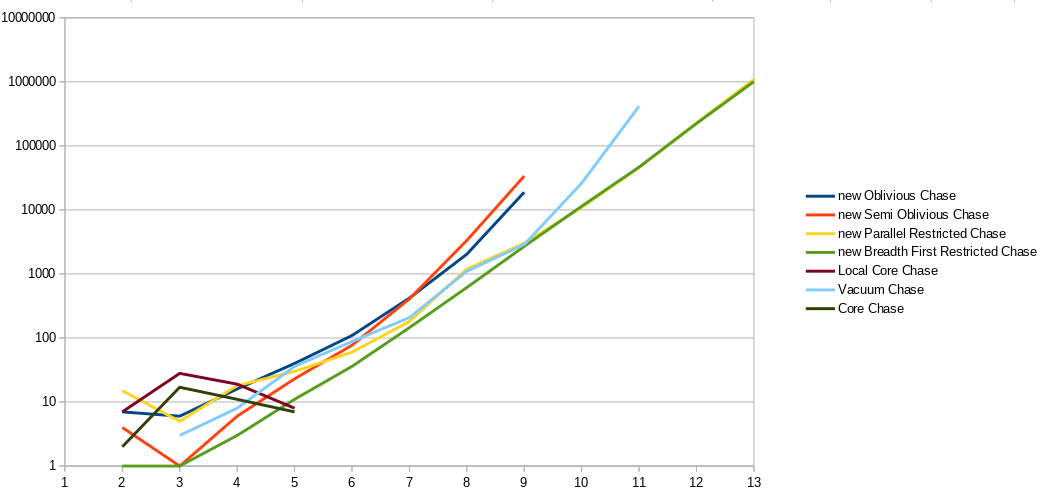
\includegraphics[width=0.9\textwidth]{img/ex0_exec_times.png}
    }
    \only<3>{
        %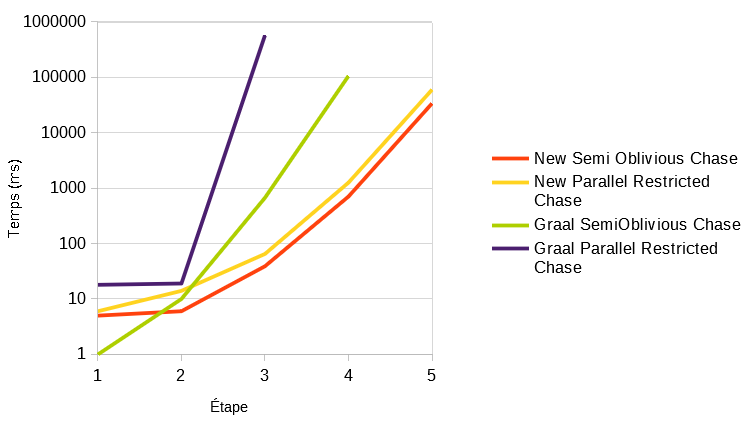
\includegraphics[width=0.7\textwidth]{img/ex11oldnew.png}
        \begin{table}[H]
\begin{center}
\begin{tabular}{|c|c|c|c|c|} 
    \hline
    $\mathcal{KB}$/Étape & \shortstack{New \\ Semi-oblivious}  & \shortstack{Graal \\ Semi-oblivious} & \shortstack{New \\ Restricted} & \shortstack{Graal \\ Restricted} \\
    \hline
     \hline
    $\mathcal{KB}_A$/6 & 55987 & 55987 & 1375 & 1375 \\ 
     \hline
    $\mathcal{KB}_B$/5 & 111111 & 111111 & 3851 & 3851 \\ 
    \hline
    $\mathcal{KB}_C$/4 & 107754 & 107754 & 21882 & 21882 \\ 
    \hline
    $\mathcal{KB}_D$/4 & \color{green}1556 & \color{green}1556 & \color{green}1556 & \color{red}152324 \\
    \hline
    $\mathcal{KB}_E$/13 & 754 & 754 & 332 & 332 \\ 
     \hline
    $\mathcal{KB}_F$/4 & 48315 & 48315 & 24918 & 24918 \\ 
     \hline 
\end{tabular}    
\caption {Comparaison des \textit{chases} par nombr \label{tab:faitsoldnew}
\end{center}
\end{table}
    }
    \end{center}
\end{frame}

